\subsection{Problema a resolver}

El siguiente ejercicio se da en el contexto de un museo donde se requiere, por cuestiones de seguridad, colocar sensores de forma tal que todo el piso del museo esté cubierto por los laser que emiten, existen dos tipos de sensores, lo direccionales (que emiten señales horizontales o verticales) y los bidireccionales (que emiten señales hacia ambos lados) y su valor es \$4000 y \$6000 respectivamente. Se pide también que un sensor no este apuntando hacia otro por que esto podria provocar que algún sensor deje de funcionar y no es lo deseado, ademas se pide que en ciertos lugares, definidos como "importantes", haya dos laser pasando simulateamente. El objetivo entonces es encontrar la forma de colocar estos sensores de forma tal que el suelo quede completamente cubierto y que los lugares importantes queden con ambos laser pasando por el y ademas que el costo total de los sensores sea minimo, tambien hay que tener en cuenta que en el museo puede haber paredes que interfieran en los laser de los sensores.

Un ejemplo de este problema es el que está provisto por la catedra


\begin{figure}[H]
	\begin{center}
		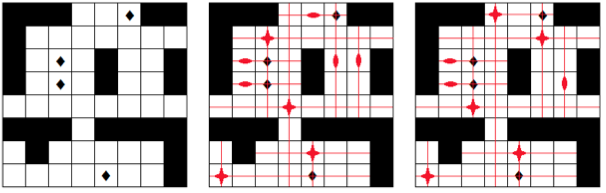
\includegraphics[width=320pt]{../imgs/ej3_ejemploCatedra.png}
	\end{center}
\caption{Un ejemplo y dos soluciones distintas.}
\end{figure}

En el ejemplo de la Figura 1 el museo se ve representado por una cuadricula donde donde los cuadrados blancos representan el suelo, los cuadrados negros representan las paredes y los cuadrados que tienen un rombo dentro representan los lugares importantes, a continuacion de la imagen se muetran dos posibles soluciones al problema, en las cuales las cruces rojas representan los sensores bidireccionales, y las lineas rojas gruesas representan los sensores horizontales y verticales, desde estos sensores se extienden lineas rojas que representan el area que cubren estos sensores.

En el primer caso el costo total es de \$44000 y la segunda solucion tiene un costo de \$42000

\subsection{Resolución coloquial}

Para resolver este ejercicio usamos, como recomendacion de la catedra en el enunciado, la técnica de backtracking que consiste en probar todas las posibles combinaciones de soluciones dentro del problema hasta llegar a las validas y guardar así la mejor de ellas usando en casa paso, criterios de parada que nos permitan deducir si las soluciones parcialmente obtenidas son candidatas a mejores soluciones o si son soluciones validas.

El modelo de nuestro problema mapea las el piso, las paredes y los lugares importantes del museo en casillas dentro de una matriz.

Para resolver el problema recorremos la matriz secuencialmente y cada paso tomamos una decision sobre el casillero actual, siento estas colocar un sensor o dejar el casillero sin ningun sensor, esta genera un arbol de decisiones en el cual cada una de sus ramas representan un escenario diferente en la distribucion de sensores en la matriz que representa nuestra modelo, de esta manera nos garantizamos obtener todas las posibles combinaciones de configuraciones de la matriz.

\subsection{Demostración de correctitud}

Sea $C$ el conjunto de configuraciones posibles de la matriz, si en cada paso puedo probar 4 configuraciones diferentes para cada casillero disponible, y si mi matriz mide $n*m$, entonces por combinatoria tengo $4^{n*m}$ configuraciones finales posilbes de la matriz, como nuestro algoritmo hace esencialmente eso (excepto por las podas y criterios de terminacion que no representan soluciones validas) podemos decir que este encuentra todas las posibles configuraciones de la matriz.

Sea $s$ una solucion optima al problema, ya que $s$ representa una configuracion particular de la matriz entonces como $C$ representa el conjunto de todas las posibles soluciones del problema y la solucion optima, si es que existe alguna solucion, está dentro de ese conjunto, entonces nuestro algoritmo deberia encontrarla y devolverla.

Es correcto por que usa backtracking.-

\subsection{Complejidad del algoritmo}

Pseudocódigo:

\begin{algorithm}[H]
	\SetAlgoLined
	\caption{Algoritmo de Backtracking}
	\KwIn{Matriz $grilla$}
	\KwOut{lista sensores}
	
	Lista $casillasLibres\ \leftarrow$ ObtenerPosicionesLibres(grilla)\\

	\For{Posicion $p \in grilla$}{
		\If{p es importante}{
			RestringirPorImportantes(p)\\
		}
	}

	sensores := backtrack($grilla$, $casillasLibres$)\\

	\textbf{devolver} sensores
\end{algorithm}

\begin{algorithm}[H]
	\SetAlgoLined
	\caption{backtrack}
	\KwIn{Matriz $grilla$, Lista $casillasLibres$}
	\KwOut{}
	
	Lista $casillaActual$ := Proxima casilla libre en casillasLibres\\

	\If{Puedo poner un sensor bidireccional en $casillaActual$}{
		Restringir por laser bidireccional\\
		Saco casillaActual de casillasLibres\\
		backtrack($grilla$, $casillasLibres$)\\
	}
	\If{Puedo poner un sensor vertical en $casillaActual$}{
		Restringir por laser vertical\\
		Restringir casilleros horizontales\\
		Saco casillaActual de casillasLibres\\
		backtrack($grilla$, $casillasLibres$)\\
	}
	\If{Puedo poner un sensor horizontal en $casillaActual$}{
		Restringir por laser horizontal\\
		Restringir casilleros verticales\\
		Saco casillaActual de casillasLibres\\
		backtrack($grilla$, $casillasLibres$)\\
	}

	Dejo el casillero en blanco\\
	backtrack($grilla$, $casillasLibres$)\\

	\textbf{devolver} ContarSensores($grilla$)
\end{algorithm}

\subsection{Código fuente}

\subsection{Instancias posibles}
Para verificar la correctitud de nuestro programa, dispusimos variar estratégicamente las instancias de entrada al ejecutarlo.
\begin{itemize}
\item En primer lugar, ejecutamos el programa ingresando un único espacio libre el cual contenía un lugar importante. La idea de esto es comprobar que nuestro algoritmo devuelve -1 en el caso de que no haya solución ya que el espacio especial no podia ser cubierto por 2 laser's.\newline

\textbf{Parámetro de entrada:} 
$$3\ \ 3$$
$$0\ \ 0\ \ 0$$
$$0\ \ 2\ \ 0$$
$$0\ \ 0\ \ 0$$
\textbf{Parámetro de salida:} $$4\ \ 1\ \ 2\ \ 3\ \ 4$$\newline
\item Por otra parte, probamos el programa cuando todo el museo es una pared y no contiene ni espacios libres ni espacios importantes, en otras palabras, el caso vacio. Lo interesante de esto es ver que nuestro algoritmo funciona en dicho caso borde.\newline

\textbf{Parámetro de entrada:} 
$$3\ \ 3$$
$$0\ \ 0\ \ 0$$
$$0\ \ 0\ \ 0$$
$$0\ \ 0\ \ 0$$
\textbf{Parámetro de salida:} $$ 0 $$\newline
\item Un caso interesante, es ver cuando todos los espacios estan libres. La idea de esto es comprobar que el algoritmo nos da la solucion mas barata al problema\newline

\textbf{Parámetro de entrada:} 
$$3\ \ 3$$
$$1\ \ 1\ \ 1$$
$$1\ \ 1\ \ 1$$
$$1\ \ 1\ \ 1$$
\textbf{Parámetro de salida:} $$ 0 $$\newline

\item Otro caso interesante, es ver cuando todos los espacios son importantes. Este es un caso particular en el cual no existe solución ya que no podrian pasar dos laser's por el mismo punto especial sin que uno de estos toque a otro laser\newline

\textbf{Parámetro de entrada:} 
$$3\ \ 3$$
$$2\ \ 2\ \ 2$$
$$2\ \ 2\ \ 2$$
$$2\ \ 2\ \ 2$$
\textbf{Parámetro de salida:} $$ 1\ \ 1 $$\newline

\item Otro caso interesante, es ir alternando piso y pared.
\textbf{Parámetro de entrada:} 
$$3\ \ 3$$
$$1\ \ 0\ \ 1$$
$$0\ \ 1\ \ 0$$
$$1\ \ 0\ \ 1$$
\textbf{Parámetro de salida:} $$ 0 $$\newline


\item Por ultimo, esta el caso en el que tenemos los 3 tipos de casilleros, este seria el caso mas comun del problema. \newline

\textbf{Parámetro de entrada:} 
$$3\ \ 3$$
$$1\ \ 1\ \ 1$$
$$1\ \ 2\ \ 0$$
$$0\ \ 0\ \ 1$$
\textbf{Parámetro de salida:} $$3\ \ 1\ \ 2\ \ 3$$\newline
\end{itemize}

\subsection{Testing}


